\subsection{Gestionar Tipo de Contacto}
%IUGestPerfiles
\subsubsection{Objetivo}
	El mapa de navegación se muestra en la Figura~\ref{fig:mapaNavegacionCUA24}

  \begin{figure}[hbpt!]
 		\centering
 			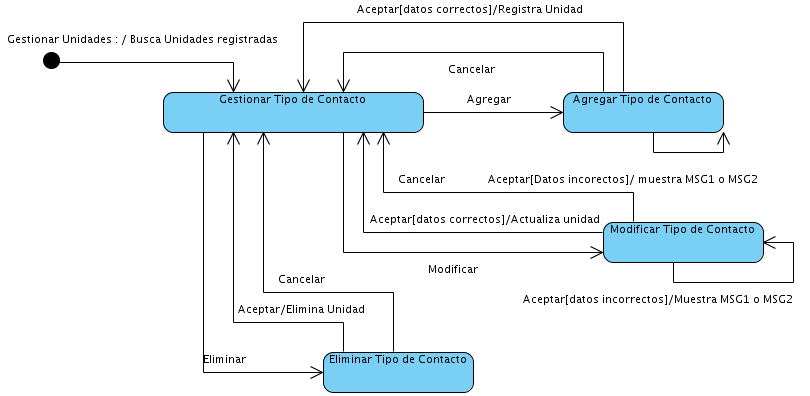
\includegraphics[width=0.8\textwidth]{images/CUA24/MapaNavegacion.png}
 		\caption{Mapa de navegacion para el CUA 24 Gestion de Tipo de Contactos.}
		\label{fig:mapaNavegacionCUA24}
 	\end{figure}

\subsubsection{Objetivo}
Mostrar el menú para agregar, modificar o eliminar un Tipo de Contacto.
Figura~\ref{IUGestTipoContacto}

\IUfig[0.5]{CUA24/GestionTipoContacto.png}{IUGestTipoContacto}{Gestionar Tipo de Contacto.}
%IUPCAdminTdU es el identificador par ala referencia
\subsubsection{Salidas}
Tipos de Contacto registrados.

%\subsubsection{Controles}

\subsubsection{Entradas}
Ninguna.


\subsubsection{Comandos}
\begin{itemize}
 \item \IUbutton{Agregar Tipo Contacto} Esta opción permite agregar un Tipo de Contacto  nuevo, al oprimirlo muestra la ventana \IUref{IUAgregarTipoContacto}{Agregar Tipo de Contacto}.
 \item \IUbutton{
\includegraphics[scale=0.1]{images/icons/editar.png}} Esta opción permite realizar modificaciones en un Tipo de Contacto, al oprimirlo muestra la ventana \IUref{IUModificarTipoContacto}{Modificar Tipo de Contacto}.
 \item \IUbutton{
\includegraphics[scale=0.1]{images/icons/eliminar.png}} Esta opción permite Eliminar un Tipo de Contacto, al oprimirlo muestra la ventana \IUref{IUEliminarTipoContacto}{Eliminar Tipo de Contacto}.

\end{itemize}


